% A0 portrait poster — Academia Sinica ISS Summer Internship 2026
% Compile with pdfLaTeX on Overleaf. Requires fig1_arch.pdf, fig2_tree.pdf in project.
\documentclass[final]{beamer}
\usepackage[orientation=portrait,size=a0,scale=1.33]{beamerposter}
\usepackage{booktabs}
\usepackage{graphicx}
\usepackage{amsmath}
\usepackage{array}

% ---------- colors ----------
\definecolor{main}{RGB}{16,46,88}      % deep navy
\definecolor{accent}{RGB}{166,30,38}   % dark red
\definecolor{lightbg}{RGB}{242,244,248}
\definecolor{midgray}{RGB}{90,96,104}

\setbeamercolor{background canvas}{bg=white}
\setbeamercolor{block title}{fg=white,bg=main}
\setbeamercolor{block body}{fg=black,bg=lightbg}
\setbeamerfont{block title}{series=\bfseries,size=\large}
\setbeamertemplate{navigation symbols}{}
\setbeamertemplate{caption}[numbered]

% tighter blocks
\setbeamertemplate{block begin}{
  \begin{beamercolorbox}[ht=3.2ex,dp=1.2ex,leftskip=0.6em,colsep*=.75ex]{block title}
    \usebeamerfont{block title}\insertblocktitle
  \end{beamercolorbox}
  \nointerlineskip
  \begin{beamercolorbox}[leftskip=0.6em,rightskip=0.6em,colsep*=.75ex,sep=0.7ex,vmode]{block body}
}
\setbeamertemplate{block end}{\end{beamercolorbox}\vspace{1.6ex}}

\newcommand{\highlight}[1]{\textcolor{accent}{\textbf{#1}}}

\begin{document}
\begin{frame}[t]

% =================== HEADER ===================
\begin{center}
  \vspace{0.6cm}
  {\VERYHuge\bfseries\textcolor{main}{Benchmarking AI Agents for Kaggle Competitions}}\\[0.5ex]
  {\Huge\bfseries\textcolor{main}{A Fair Three-Way Comparison with Paired Significance Testing}}\\[1.2ex]
  {\LARGE Wei-Hao Huang}\\[0.6ex]
  {\Large National Chengchi University, Department of Economics (Double Major: Applied Mathematics)}\\[0.4ex]
  {\Large Advisor: Dr.\ Tso-Jung Yen --- Institute of Statistical Science, Academia Sinica}\\[0.4ex]
  {\large 2026 Summer Internship Program}
  \vspace{0.4cm}
\end{center}
\vspace{-0.2cm}
{\color{main}\hrule height 3pt}
\vspace{0.8cm}

% =================== BODY: 3 columns ===================
\begin{columns}[t]

% ---------------- COLUMN 1 ----------------
\begin{column}{0.315\textwidth}

\begin{block}{1~~Motivation}
LLM-driven agents can now solve Kaggle competitions end-to-end, but the methodology for comparing them is weak --- \emph{one run, one score, higher wins}.
\begin{itemize}
  \item \highlight{Q1 --- Positioning.} Where does our own agent stand? Self-assessment without external, methodologically different reference points is circular.
  \item \highlight{Q2 --- Noise.} Competition metrics carry sampling error and agent runs are stochastic. In how many competitions can agents \emph{actually} be told apart?
\end{itemize}
\end{block}

\begin{block}{2~~Three distinct agents}
\centering
\small
\begin{tabular}{@{}p{0.24\linewidth}p{0.24\linewidth}p{0.20\linewidth}p{0.22\linewidth}@{}}
\toprule
 & \textbf{my-agent} & \textbf{AIDE} & \textbf{NVIDIA} \\
\midrule
Knowledge & experience library (accumulates) & none (cold start) & public kernels \\
Search & 6-stage + tree search, 25--80 nodes & LLM tree search, 20 steps & no search: reproduce \\
Validation & split by task type; diagnostics quarantined & no split legality & inherits kernel's \\
External data & proactively joined & never & inherited \\
\bottomrule
\end{tabular}

\vspace{0.8ex}
\raggedright
\textbf{my-agent} is our hybrid design (Claude Code Skill): the LLM reasons and decides; LightGBM/XGBoost/CatBoost/Optuna execute. Both reference methods are \highlight{frozen} --- improving a yardstick mid-study would corrupt the comparison.
\end{block}

\begin{block}{3~~my-agent architecture}
\centering

\includegraphics[width=0.97\linewidth]{fig1_arch.pdf}
\vspace{0.4ex}
\raggedright\small
The experience library only stores insights carrying a \emph{score-delta evidence field}; validated insights flow back for future competitions.
\end{block}

\begin{block}{4~~Tree-search loop (harness v3)}
\centering
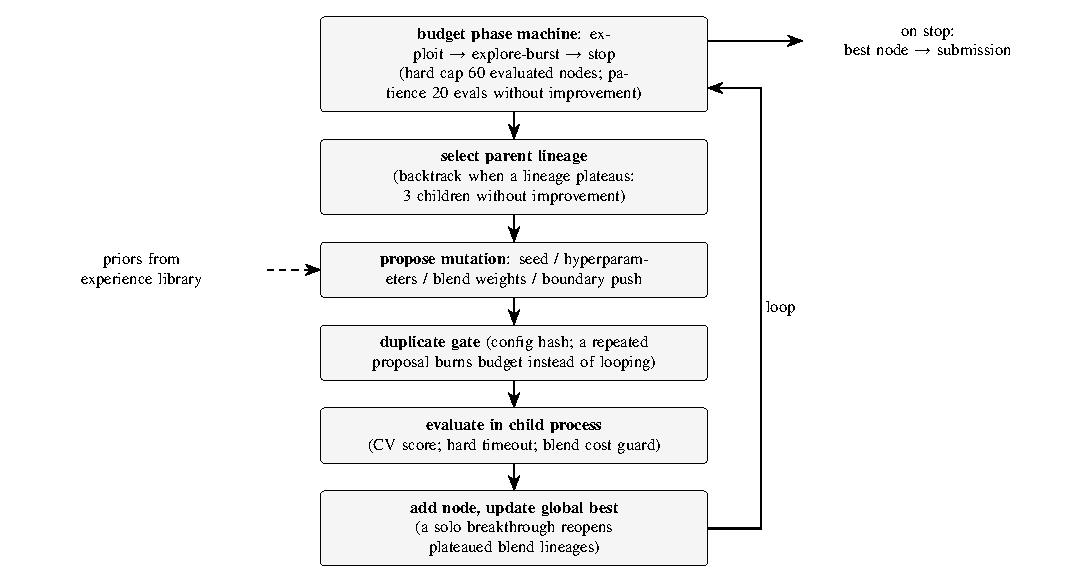
\includegraphics[width=0.8\linewidth]{fig2_tree.pdf}
\end{block}

\end{column}

% ---------------- COLUMN 2 ----------------
\begin{column}{0.315\textwidth}

\begin{block}{5~~A fair benchmark: 18 competitions}
\textbf{Evaluation set.} 13 Kaggle Playground competitions + 5 non-Playground (afsis 2014, conway 2014, cat-in-the-dat 2019, tps-aug/jan-2022). Inclusion criterion: both public and private leaderboard scores available. Every submission is scored on the \emph{real} leaderboard via late submission.

\vspace{0.6ex}
\textbf{Mechanically enforced fairness} (three agents, one machine):
\begin{itemize}
  \item \textbf{Data isolation} --- manifest-validated isolated roots
  \item \textbf{Resource isolation} --- mutex: one lane at a time
  \item \textbf{Instruction isolation} --- prompts carry no recipes, no other agent's findings; environment defects are fixed, never hinted
\end{itemize}
\end{block}

\begin{block}{6~~The paired significance test}
Kaggle scores one submission on two disjoint test subsets --- two independent estimates of the same model. Their gap is that competition's \emph{sampling noise}.

\vspace{0.6ex}
\textbf{Naive thresholds fail.} An agent's own public--private drift is \emph{shared}: on s5e10 the three drifts are $+0.00025/+0.00026/+0.00024$ --- common shift $0.00025$, mutual scatter only $\mathbf{0.00002}$. Using it as a threshold inflates noise $>$10$\times$.

\vspace{0.6ex}
\textbf{The paired construction.} For the between-agent gap $d$, a verdict requires:
\begin{align*}
\operatorname{sign}(d_{\text{priv}}) &= \operatorname{sign}(d_{\text{pub}}) && \text{order replicates}\\
|d_{\text{priv}}| &> |d_{\text{priv}} - d_{\text{pub}}| && \text{gap exceeds its own movement}
\end{align*}
Common drift cancels in the subtraction. No extra experiments needed.
\end{block}

\begin{block}{7~~Results: 54 duels, 40 decidable}
\centering
\begin{tabular}{@{}lccc@{}}
\toprule
 & \textbf{Wins} & \textbf{Losses} & \textbf{Win rate} \\
\midrule
\textbf{my-agent} & 16 & 11 & \highlight{59\%} \\
AIDE & 11 & 13 & 46\% \\
NVIDIA & 13 & 16 & 45\% \\
\midrule
Ties & \multicolumn{3}{c}{14 duels \highlight{(26\%)}} \\
\bottomrule
\end{tabular}

\vspace{0.8ex}
\raggedright
Median percentile rank vs.\ all human teams: my-agent \textbf{72.3}, AIDE 70.8, NVIDIA 66.7. \highlight{A quarter of all duels are statistically undecidable} --- a naive tally would report that fraction as conclusions.
\end{block}

\begin{block}{8~~Local CV vs.\ the leaderboard}
CV-based and leaderboard-based conclusions \highlight{disagree in 10 of 13} comparable competitions. Extreme case (s3e19, SMAPE):
\begin{center}
\small
\begin{tabular}{@{}lccl@{}}
\toprule
Basis & my-agent & NVIDIA & Verdict \\
\midrule
Local CV & 10.02 & 13.72 & my-agent wins big \\
Private LB & 50.46 & 48.27 & NVIDIA wins \\
\bottomrule
\end{tabular}
\end{center}
The direction fully reverses: agent benchmarks must submit to the real leaderboard.
\end{block}

\end{column}

% ---------------- COLUMN 3 ----------------
\begin{column}{0.315\textwidth}

\begin{block}{9~~Ranking $=$ method $\times$ evaluation set}
Same agents, same test --- swap the competition set and the ranking \highlight{fully reverses}:
\begin{center}
\begin{tabular}{@{}lccc@{}}
\toprule
\textbf{Win rate on} & \textbf{my-agent} & \textbf{AIDE} & \textbf{NVIDIA} \\
\midrule
Playground subset (13) & 44\% (last) & 47\% & \textbf{58\%} (first) \\
Full baseline (18) & \textbf{59\%} (first) & 46\% & 45\% (last) \\
\bottomrule
\end{tabular}
\end{center}
\vspace{0.5ex}
Mechanism: the 5 non-Playground competitions are old or niche --- no mature public kernels, so NVIDIA's reproduction strategy loses its precondition (PR drops to 18.8 on afsis). Median PR, in contrast, orders the three identically on both sets. \textbf{``Which agent is stronger'' is incomplete --- the question is \emph{on what distribution of competitions}.}
\end{block}

\begin{block}{10~~Failure modes}
\begin{itemize}
  \item \highlight{AIDE: diagnosis cannot veto the score.} On s3e19 an unrelated bug fix silently switched validation to shuffled KFold: metric jumped $18.4 \to 4.4$. Controlled experiment: same features, same model, split changed only --- \textbf{4.5$\times$ optimism bias} (4.56 vs.\ 20.41). AIDE spent 9 steps tuning a leaked metric. my-agent hit the same trap but tagged it ``DIAGNOSTIC: not for submission.''
  \item \highlight{NVIDIA: votes $\neq$ quality.} An 89-vote workhorse kernel beat all three agents; a 7{,}859-vote tutorial kernel came last. Nothing checks the reproduced score against the source's claimed rank.
  \item \highlight{Shared gap:} none of the three recognizes ``this task needs external data'' (s3e19 requires GDP data; all three landed in the bimodal leaderboard's lower mode).
\end{itemize}
\end{block}

\begin{block}{11~~Conclusions}
\begin{enumerate}
  \item A credible 3-way comparison on 18 competitions: my-agent 59\% / AIDE 46\% / NVIDIA 45\%, with 26\% of duels undecidable.
  \item A \textbf{paired significance test} for agent benchmarks whose error scale comes free from Kaggle's public/private split.
  \item Local CV disagrees with the real leaderboard in 10/13 competitions --- CV-only agent benchmarks are unreliable.
  \item Benchmark claims must state the \textbf{evaluation-set composition} and report both absolute (percentile) and relative (paired win rate) metrics.
\end{enumerate}
\end{block}

\begin{block}{12~~Ongoing work}
Between-run variance of AIDE (repeatability re-runs on the 5 closest competitions); extension to NLP / time-series / imaging competitions; validation gates that let diagnoses veto scores; experience-library ablation.
\end{block}

\vspace{0.4ex}
{\small\color{midgray} Code, experiment logs, and per-competition ML specification reports: \texttt{github.com/930731haohao-afk/kaggle-agent} (private; access on request). Every number is traceable to structured experiment records.}

\end{column}

\end{columns}
\end{frame}
\end{document}
